\subsection{Шестое БДЗ}

\i\textbf{8}\\
$f(x) = \frac{\sin x}{x},\ x_0 = \frac{\pi}{2}$.\\
$f(x) = f(x_0) + \frac{f\hatch(x_0)}{1!}(x-x_0) + \frac{f\hatch\hatch(x_0)}{2!}(x-x_0)^2 + \frac{f\hatch\hatch\hatch(x_0)}{3!}(x-x_0)^3 + \oo((x-x_0)^3);$\\
$f(x) = \frac{2}{\pi} - \frac{4}{\pi^2}(x-\frac{\pi}{2}) + \frac{8-\pi^2}{\pi^3}(x-\frac{\pi}{2})^2 + \frac{2(\pi^2-8)}{\pi^4}(x-\frac{\pi}{2})^3 + \oo((x-\frac{\pi}{2})^3);$

\i\textbf{6}\\
$f(x) = \cos x,\ x_0 = \frac{\pi}{3};$\\
$\letus y = x - \frac{\pi}{3},\ y_0 = 0:$\\
$f(y) = 1 - \frac{1}{2!}y^2 + \frac{1}{4!}y^4 + \ldots + (-1)^{\floor{\frac{n}{2}}}\frac{1}{(2\floor{\frac{n}{2}})!}y^{2\floor{\frac{n}{2}}} + \oo(y^n);$\\
$f(x) = 1 - \frac{1}{2!}(x-\frac{\pi}{3})^2 + \frac{1}{4!}(x-\frac{\pi}{3})^4 + \ldots + (-1)^{\floor{\frac{n}{2}}}\frac{1}{(2\floor{\frac{n}{2}})!}(x-\frac{\pi}{3})^{2\floor{\frac{n}{2}}} + \oo((x-\frac{\pi}{3})^n);$


\i\textbf{1}\\
Рассмотрим функцию $e^x$, тогда её остаточный член в форме Лагранжа при записи многочлена Тейлора в нуле до $n$-той степени будет иметь вид $\frac{e^c}{(n+1)!}x^{n+1}$. При этом $x = \frac{1}{3}$. Нам хочется, чтобы $\frac{e^c}{(n+1)!}x^{n+1} \leq \frac{e^{\frac{1}{3}}}{(n+1)!}\brackets{\frac{1}{2}}^{n+1} < \frac{4^{\frac{1}{3}}}{(n+1)!}\brackets{\frac{1}{3}}^{n+1}$ было меньше $0{,}001$, что верно, начиная с $n=3$. Значит нам достаточно расписать только первые 4 члена многочлена Лагранжа.\\
$\sqrt[3]{e} \approx 1 + \frac{1}{1!}\frac{1}{3} + \frac{1}{2!}\brackets{\frac{1}{3}}^2 + \frac{1}{3!}\brackets{\frac{1}{3}}^3 \approx 1{,}39506$.

\i\textbf{1}\\
\begin{gather*}
    \limit{x}{0}\frac{e^{\tg x}-x}{\ln(x^2+1)-x^2} = \limit{x}{0} \frac{1}{\ln(x^2+1)-x^2} = \limit{x}{0} \frac{1}{-\frac{x^4}{2} + \frac{x^6}{3} + \ldots + (-1)^{n+1}\frac{x^{2n}}{n} + \ldots} = \\
    = \limit{x}{0}\frac{1}{-0} = -\infty;
\end{gather*}

\i\textbf{8}\\
\pu $f(x) = \frac{e^{3x-5}}{3x-5}$. Числитель всегда больше нуля, поэтому функция не имеет нулей, $\frac{5}{3}$ "--- точка разрыва. $f\hatch(x) = \frac{9e^{3x-5}(x-2)}{(3x-5)^2}$. Ноль первой производной "--- $x=2$. $f\hatch\hatch(x) = \frac{9e^{3x-5}(9x^2-36x+37)}{(3x-5)^3}$. Вторая производная не имеет нулей. Точка минимума "--- $(2, e)$, точка разрыва "--- $x=\frac{5}{3}$, при этом $\limit{x}{\frac{5}{3}-}=-\infty$, $\limit{x}{\frac{5}{3}+} = +\infty$. Тогда построим график.

\pgfplotsset{compat=1.15}
\usetikzlibrary{arrows}
\pagestyle{empty}
 
%<<<<<<<WARNING>>>>>>>
% PGF/Tikz doesn't support the following mathematical functions:
% cosh, acosh, sinh, asinh, tanh, atanh,
% x^r with r not integer

% Plotting will be done using GNUPLOT
% GNUPLOT must be installed and you must allow Latex to call external
% programs by adding the following option to your compiler
% shell-escape    OR    enable-write18 
% Example: pdflatex --shell-escape file.tex 

\definecolor{qqwuqq}{rgb}{0,0.39215686274509803,0}
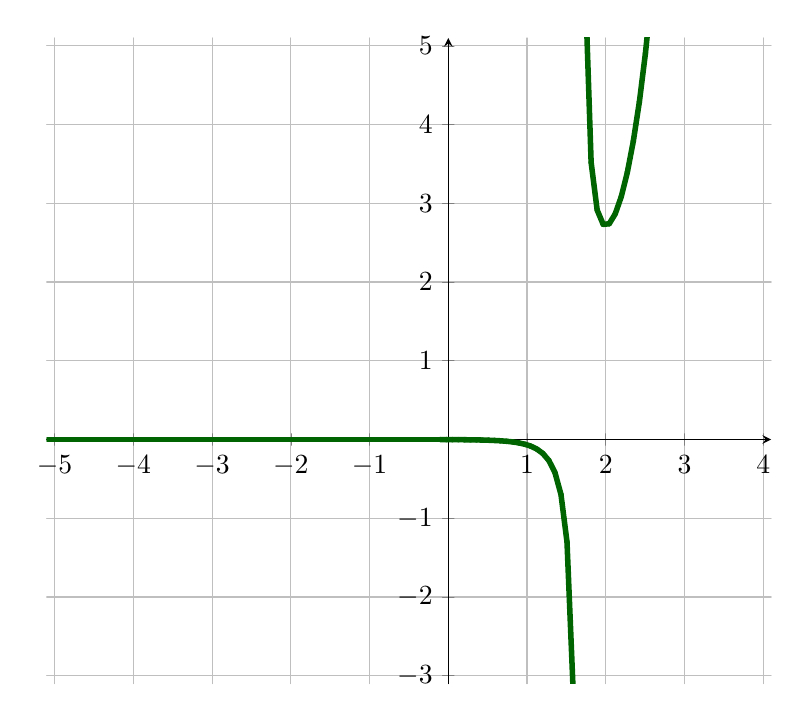
\begin{tikzpicture}[line cap=round,line join=round,>=triangle 45,x=1cm,y=1cm]
\begin{axis}[
x=1cm,y=1cm,
axis lines=middle,
ymajorgrids=true,
xmajorgrids=true,
xmin=-5.1,
xmax=4.1,
ymin=-3.1,
ymax=5.1,
xtick={-12,-11,...,17},
ytick={-8,-7,...,11},]
\clip(-12.74,-8.82) rectangle (17.9,11.26);
\draw[line width=2pt,color=qqwuqq] (-12.74,0) -- (-12.74,0);
\draw[line width=2pt,color=qqwuqq] (-12.74,0) -- (-12.6634,0);
\draw[line width=2pt,color=qqwuqq] (-12.6634,0) -- (-12.586799999999998,0);
\draw[line width=2pt,color=qqwuqq] (-12.586799999999998,0) -- (-12.510199999999998,0);
\draw[line width=2pt,color=qqwuqq] (-12.510199999999998,0) -- (-12.433599999999997,0);
\draw[line width=2pt,color=qqwuqq] (-12.433599999999997,0) -- (-12.356999999999996,0);
\draw[line width=2pt,color=qqwuqq] (-12.356999999999996,0) -- (-12.280399999999995,0);
\draw[line width=2pt,color=qqwuqq] (-12.280399999999995,0) -- (-12.203799999999994,0);
\draw[line width=2pt,color=qqwuqq] (-12.203799999999994,0) -- (-12.127199999999993,0);
\draw[line width=2pt,color=qqwuqq] (-12.127199999999993,0) -- (-12.050599999999992,0);
\draw[line width=2pt,color=qqwuqq] (-12.050599999999992,0) -- (-11.973999999999991,0);
\draw[line width=2pt,color=qqwuqq] (-11.973999999999991,0) -- (-11.89739999999999,0);
\draw[line width=2pt,color=qqwuqq] (-11.89739999999999,0) -- (-11.82079999999999,0);
\draw[line width=2pt,color=qqwuqq] (-11.82079999999999,0) -- (-11.744199999999989,0);
\draw[line width=2pt,color=qqwuqq] (-11.744199999999989,0) -- (-11.667599999999988,0);
\draw[line width=2pt,color=qqwuqq] (-11.667599999999988,0) -- (-11.590999999999987,0);
\draw[line width=2pt,color=qqwuqq] (-11.590999999999987,0) -- (-11.514399999999986,0);
\draw[line width=2pt,color=qqwuqq] (-11.514399999999986,0) -- (-11.437799999999985,0);
\draw[line width=2pt,color=qqwuqq] (-11.437799999999985,0) -- (-11.361199999999984,0);
\draw[line width=2pt,color=qqwuqq] (-11.361199999999984,0) -- (-11.284599999999983,0);
\draw[line width=2pt,color=qqwuqq] (-11.284599999999983,0) -- (-11.207999999999982,0);
\draw[line width=2pt,color=qqwuqq] (-11.207999999999982,0) -- (-11.131399999999982,0);
\draw[line width=2pt,color=qqwuqq] (-11.131399999999982,0) -- (-11.05479999999998,0);
\draw[line width=2pt,color=qqwuqq] (-11.05479999999998,0) -- (-10.97819999999998,0);
\draw[line width=2pt,color=qqwuqq] (-10.97819999999998,0) -- (-10.901599999999979,0);
\draw[line width=2pt,color=qqwuqq] (-10.901599999999979,0) -- (-10.824999999999978,0);
\draw[line width=2pt,color=qqwuqq] (-10.824999999999978,0) -- (-10.748399999999977,0);
\draw[line width=2pt,color=qqwuqq] (-10.748399999999977,0) -- (-10.671799999999976,0);
\draw[line width=2pt,color=qqwuqq] (-10.671799999999976,0) -- (-10.595199999999975,0);
\draw[line width=2pt,color=qqwuqq] (-10.595199999999975,0) -- (-10.518599999999974,0);
\draw[line width=2pt,color=qqwuqq] (-10.518599999999974,0) -- (-10.441999999999974,0);
\draw[line width=2pt,color=qqwuqq] (-10.441999999999974,0) -- (-10.365399999999973,0);
\draw[line width=2pt,color=qqwuqq] (-10.365399999999973,0) -- (-10.288799999999972,0);
\draw[line width=2pt,color=qqwuqq] (-10.288799999999972,0) -- (-10.21219999999997,0);
\draw[line width=2pt,color=qqwuqq] (-10.21219999999997,0) -- (-10.13559999999997,0);
\draw[line width=2pt,color=qqwuqq] (-10.13559999999997,0) -- (-10.058999999999969,0);
\draw[line width=2pt,color=qqwuqq] (-10.058999999999969,0) -- (-9.982399999999968,0);
\draw[line width=2pt,color=qqwuqq] (-9.982399999999968,0) -- (-9.905799999999967,0);
\draw[line width=2pt,color=qqwuqq] (-9.905799999999967,0) -- (-9.829199999999966,0);
\draw[line width=2pt,color=qqwuqq] (-9.829199999999966,0) -- (-9.752599999999966,0);
\draw[line width=2pt,color=qqwuqq] (-9.752599999999966,0) -- (-9.675999999999965,0);
\draw[line width=2pt,color=qqwuqq] (-9.675999999999965,0) -- (-9.599399999999964,0);
\draw[line width=2pt,color=qqwuqq] (-9.599399999999964,0) -- (-9.522799999999963,0);
\draw[line width=2pt,color=qqwuqq] (-9.522799999999963,0) -- (-9.446199999999962,0);
\draw[line width=2pt,color=qqwuqq] (-9.446199999999962,0) -- (-9.369599999999961,0);
\draw[line width=2pt,color=qqwuqq] (-9.369599999999961,0) -- (-9.29299999999996,0);
\draw[line width=2pt,color=qqwuqq] (-9.29299999999996,0) -- (-9.21639999999996,0);
\draw[line width=2pt,color=qqwuqq] (-9.21639999999996,0) -- (-9.139799999999958,0);
\draw[line width=2pt,color=qqwuqq] (-9.139799999999958,0) -- (-9.063199999999958,0);
\draw[line width=2pt,color=qqwuqq] (-9.063199999999958,0) -- (-8.986599999999957,0);
\draw[line width=2pt,color=qqwuqq] (-8.986599999999957,0) -- (-8.909999999999956,0);
\draw[line width=2pt,color=qqwuqq] (-8.909999999999956,0) -- (-8.833399999999955,0);
\draw[line width=2pt,color=qqwuqq] (-8.833399999999955,0) -- (-8.756799999999954,0);
\draw[line width=2pt,color=qqwuqq] (-8.756799999999954,0) -- (-8.680199999999953,0);
\draw[line width=2pt,color=qqwuqq] (-8.680199999999953,0) -- (-8.603599999999952,0);
\draw[line width=2pt,color=qqwuqq] (-8.603599999999952,0) -- (-8.526999999999951,0);
\draw[line width=2pt,color=qqwuqq] (-8.526999999999951,0) -- (-8.45039999999995,0);
\draw[line width=2pt,color=qqwuqq] (-8.45039999999995,0) -- (-8.37379999999995,0);
\draw[line width=2pt,color=qqwuqq] (-8.37379999999995,0) -- (-8.297199999999949,0);
\draw[line width=2pt,color=qqwuqq] (-8.297199999999949,0) -- (-8.220599999999948,0);
\draw[line width=2pt,color=qqwuqq] (-8.220599999999948,0) -- (-8.143999999999947,0);
\draw[line width=2pt,color=qqwuqq] (-8.143999999999947,0) -- (-8.067399999999946,0);
\draw[line width=2pt,color=qqwuqq] (-8.067399999999946,0) -- (-7.990799999999946,0);
\draw[line width=2pt,color=qqwuqq] (-7.990799999999946,0) -- (-7.914199999999946,0);
\draw[line width=2pt,color=qqwuqq] (-7.914199999999946,0) -- (-7.837599999999946,0);
\draw[line width=2pt,color=qqwuqq] (-7.837599999999946,0) -- (-7.760999999999946,0);
\draw[line width=2pt,color=qqwuqq] (-7.760999999999946,0) -- (-7.684399999999946,0);
\draw[line width=2pt,color=qqwuqq] (-7.684399999999946,0) -- (-7.607799999999946,0);
\draw[line width=2pt,color=qqwuqq] (-7.607799999999946,0) -- (-7.531199999999946,0);
\draw[line width=2pt,color=qqwuqq] (-7.531199999999946,0) -- (-7.454599999999946,0);
\draw[line width=2pt,color=qqwuqq] (-7.454599999999946,0) -- (-7.377999999999946,0);
\draw[line width=2pt,color=qqwuqq] (-7.377999999999946,0) -- (-7.301399999999946,0);
\draw[line width=2pt,color=qqwuqq] (-7.301399999999946,0) -- (-7.224799999999946,0);
\draw[line width=2pt,color=qqwuqq] (-7.224799999999946,0) -- (-7.148199999999946,0);
\draw[line width=2pt,color=qqwuqq] (-7.148199999999946,0) -- (-7.071599999999946,0);
\draw[line width=2pt,color=qqwuqq] (-7.071599999999946,0) -- (-6.994999999999946,0);
\draw[line width=2pt,color=qqwuqq] (-6.994999999999946,0) -- (-6.918399999999946,0);
\draw[line width=2pt,color=qqwuqq] (-6.918399999999946,0) -- (-6.841799999999946,0);
\draw[line width=2pt,color=qqwuqq] (-6.841799999999946,0) -- (-6.765199999999946,0);
\draw[line width=2pt,color=qqwuqq] (-6.765199999999946,0) -- (-6.688599999999946,0);
\draw[line width=2pt,color=qqwuqq] (-6.688599999999946,0) -- (-6.611999999999946,0);
\draw[line width=2pt,color=qqwuqq] (-6.611999999999946,0) -- (-6.535399999999946,0);
\draw[line width=2pt,color=qqwuqq] (-6.535399999999946,0) -- (-6.458799999999946,0);
\draw[line width=2pt,color=qqwuqq] (-6.458799999999946,0) -- (-6.382199999999946,0);
\draw[line width=2pt,color=qqwuqq] (-6.382199999999946,0) -- (-6.305599999999946,0);
\draw[line width=2pt,color=qqwuqq] (-6.305599999999946,0) -- (-6.228999999999946,0);
\draw[line width=2pt,color=qqwuqq] (-6.228999999999946,0) -- (-6.152399999999946,0);
\draw[line width=2pt,color=qqwuqq] (-6.152399999999946,0) -- (-6.075799999999946,0);
\draw[line width=2pt,color=qqwuqq] (-6.075799999999946,0) -- (-5.999199999999946,0);
\draw[line width=2pt,color=qqwuqq] (-5.999199999999946,0) -- (-5.922599999999946,0);
\draw[line width=2pt,color=qqwuqq] (-5.922599999999946,0) -- (-5.845999999999946,0);
\draw[line width=2pt,color=qqwuqq] (-5.845999999999946,0) -- (-5.769399999999946,0);
\draw[line width=2pt,color=qqwuqq] (-5.769399999999946,0) -- (-5.692799999999946,0);
\draw[line width=2pt,color=qqwuqq] (-5.692799999999946,0) -- (-5.616199999999946,0);
\draw[line width=2pt,color=qqwuqq] (-5.616199999999946,0) -- (-5.539599999999946,0);
\draw[line width=2pt,color=qqwuqq] (-5.539599999999946,0) -- (-5.462999999999946,0);
\draw[line width=2pt,color=qqwuqq] (-5.462999999999946,0) -- (-5.386399999999946,0);
\draw[line width=2pt,color=qqwuqq] (-5.386399999999946,0) -- (-5.309799999999946,0);
\draw[line width=2pt,color=qqwuqq] (-5.309799999999946,0) -- (-5.233199999999946,0);
\draw[line width=2pt,color=qqwuqq] (-5.233199999999946,0) -- (-5.156599999999946,0);
\draw[line width=2pt,color=qqwuqq] (-5.156599999999946,0) -- (-5.079999999999946,0);
\draw[line width=2pt,color=qqwuqq] (-5.079999999999946,0) -- (-5.003399999999946,0);
\draw[line width=2pt,color=qqwuqq] (-5.003399999999946,0) -- (-4.926799999999946,0);
\draw[line width=2pt,color=qqwuqq] (-4.926799999999946,0) -- (-4.850199999999946,0);
\draw[line width=2pt,color=qqwuqq] (-4.850199999999946,0) -- (-4.773599999999946,0);
\draw[line width=2pt,color=qqwuqq] (-4.773599999999946,0) -- (-4.696999999999946,0);
\draw[line width=2pt,color=qqwuqq] (-4.696999999999946,0) -- (-4.620399999999946,0);
\draw[line width=2pt,color=qqwuqq] (-4.620399999999946,0) -- (-4.543799999999946,0);
\draw[line width=2pt,color=qqwuqq] (-4.543799999999946,0) -- (-4.467199999999946,0);
\draw[line width=2pt,color=qqwuqq] (-4.467199999999946,0) -- (-4.390599999999946,0);
\draw[line width=2pt,color=qqwuqq] (-4.390599999999946,0) -- (-4.313999999999946,0);
\draw[line width=2pt,color=qqwuqq] (-4.313999999999946,0) -- (-4.237399999999946,0);
\draw[line width=2pt,color=qqwuqq] (-4.237399999999946,0) -- (-4.160799999999946,0);
\draw[line width=2pt,color=qqwuqq] (-4.160799999999946,0) -- (-4.084199999999946,0);
\draw[line width=2pt,color=qqwuqq] (-4.084199999999946,0) -- (-4.007599999999946,0);
\draw[line width=2pt,color=qqwuqq] (-4.007599999999946,0) -- (-3.930999999999946,0);
\draw[line width=2pt,color=qqwuqq] (-3.930999999999946,0) -- (-3.854399999999946,0);
\draw[line width=2pt,color=qqwuqq] (-3.854399999999946,0) -- (-3.777799999999946,0);
\draw[line width=2pt,color=qqwuqq] (-3.777799999999946,0) -- (-3.701199999999946,0);
\draw[line width=2pt,color=qqwuqq] (-3.701199999999946,0) -- (-3.624599999999946,0);
\draw[line width=2pt,color=qqwuqq] (-3.624599999999946,0) -- (-3.547999999999946,0);
\draw[line width=2pt,color=qqwuqq] (-3.547999999999946,0) -- (-3.471399999999946,0);
\draw[line width=2pt,color=qqwuqq] (-3.471399999999946,0) -- (-3.394799999999946,0);
\draw[line width=2pt,color=qqwuqq] (-3.394799999999946,0) -- (-3.318199999999946,0);
\draw[line width=2pt,color=qqwuqq] (-3.318199999999946,0) -- (-3.241599999999946,0);
\draw[line width=2pt,color=qqwuqq] (-3.241599999999946,0) -- (-3.164999999999946,0);
\draw[line width=2pt,color=qqwuqq] (-3.164999999999946,0) -- (-3.088399999999946,0);
\draw[line width=2pt,color=qqwuqq] (-3.088399999999946,0) -- (-3.011799999999946,0);
\draw[line width=2pt,color=qqwuqq] (-3.011799999999946,0) -- (-2.935199999999946,0);
\draw[line width=2pt,color=qqwuqq] (-2.935199999999946,0) -- (-2.858599999999946,0);
\draw[line width=2pt,color=qqwuqq] (-2.858599999999946,0) -- (-2.781999999999946,0);
\draw[line width=2pt,color=qqwuqq] (-2.781999999999946,0) -- (-2.705399999999946,0);
\draw[line width=2pt,color=qqwuqq] (-2.705399999999946,0) -- (-2.628799999999946,0);
\draw[line width=2pt,color=qqwuqq] (-2.628799999999946,0) -- (-2.552199999999946,0);
\draw[line width=2pt,color=qqwuqq] (-2.552199999999946,0) -- (-2.475599999999946,0);
\draw[line width=2pt,color=qqwuqq] (-2.475599999999946,0) -- (-2.398999999999946,0);
\draw[line width=2pt,color=qqwuqq] (-2.398999999999946,0) -- (-2.322399999999946,0);
\draw[line width=2pt,color=qqwuqq] (-2.322399999999946,0) -- (-2.245799999999946,0);
\draw[line width=2pt,color=qqwuqq] (-2.245799999999946,0) -- (-2.169199999999946,0);
\draw[line width=2pt,color=qqwuqq] (-2.169199999999946,0) -- (-2.092599999999946,0);
\draw[line width=2pt,color=qqwuqq] (-2.092599999999946,0) -- (-2.015999999999946,0);
\draw[line width=2pt,color=qqwuqq] (-2.015999999999946,0) -- (-1.9393999999999458,0);
\draw[line width=2pt,color=qqwuqq] (-1.9393999999999458,0) -- (-1.8627999999999458,0);
\draw[line width=2pt,color=qqwuqq] (-1.8627999999999458,0) -- (-1.7861999999999458,0);
\draw[line width=2pt,color=qqwuqq] (-1.7861999999999458,0) -- (-1.7095999999999458,0);
\draw[line width=2pt,color=qqwuqq] (-1.7095999999999458,0) -- (-1.6329999999999458,0);
\draw[line width=2pt,color=qqwuqq] (-1.6329999999999458,0) -- (-1.5563999999999458,0);
\draw[line width=2pt,color=qqwuqq] (-1.5563999999999458,0) -- (-1.4797999999999458,0);
\draw[line width=2pt,color=qqwuqq] (-1.4797999999999458,0) -- (-1.4031999999999458,0);
\draw[line width=2pt,color=qqwuqq] (-1.4031999999999458,0) -- (-1.3265999999999458,0);
\draw[line width=2pt,color=qqwuqq] (-1.3265999999999458,0) -- (-1.2499999999999458,0);
\draw[line width=2pt,color=qqwuqq] (-1.2499999999999458,0) -- (-1.1733999999999458,0);
\draw[line width=2pt,color=qqwuqq] (-1.1733999999999458,0) -- (-1.0967999999999458,0);
\draw[line width=2pt,color=qqwuqq] (-1.0967999999999458,0) -- (-1.0201999999999458,0);
\draw[line width=2pt,color=qqwuqq] (-1.0201999999999458,0) -- (-0.9435999999999458,0);
\draw[line width=2pt,color=qqwuqq] (-0.9435999999999458,0) -- (-0.8669999999999458,0);
\draw[line width=2pt,color=qqwuqq] (-0.8669999999999458,0) -- (-0.7903999999999458,0);
\draw[line width=2pt,color=qqwuqq] (-0.7903999999999458,0) -- (-0.7137999999999458,0);
\draw[line width=2pt,color=qqwuqq] (-0.7137999999999458,0) -- (-0.6371999999999458,0);
\draw[line width=2pt,color=qqwuqq] (-0.6371999999999458,0) -- (-0.5605999999999458,0);
\draw[line width=2pt,color=qqwuqq] (-0.5605999999999458,0) -- (-0.4839999999999458,0);
\draw[line width=2pt,color=qqwuqq] (-0.4839999999999458,0) -- (-0.4073999999999458,0);
\draw[line width=2pt,color=qqwuqq] (-0.4073999999999458,0) -- (-0.3307999999999458,0);
\draw[line width=2pt,color=qqwuqq] (-0.3307999999999458,0) -- (-0.2541999999999458,0);
\draw[line width=2pt,color=qqwuqq] (-0.2541999999999458,0) -- (-0.1775999999999458,0);
\draw[line width=2pt,color=qqwuqq] (-0.1775999999999458,0) -- (-0.10099999999994579,0);
\draw[line width=2pt,color=qqwuqq] (-0.10099999999994579,0) -- (-0.02439999999994577,-0.001234398117176523);
\draw[line width=2pt,color=qqwuqq] (-0.02439999999994577,-0.001234398117176523) -- (0.052200000000054245,-0.0016270008091092024);
\draw[line width=2pt,color=qqwuqq] (0.052200000000054245,-0.0016270008091092024) -- (0.12880000000005426,-0.0021493099038514445);
\draw[line width=2pt,color=qqwuqq] (0.12880000000005426,-0.0021493099038514445) -- (0.20540000000005426,-0.002846355348548337);
\draw[line width=2pt,color=qqwuqq] (0.20540000000005426,-0.002846355348548337) -- (0.28200000000005426,-0.00377984707902368);
\draw[line width=2pt,color=qqwuqq] (0.28200000000005426,-0.00377984707902368) -- (0.35860000000005426,-0.005034895494664597);
\draw[line width=2pt,color=qqwuqq] (0.35860000000005426,-0.005034895494664597) -- (0.43520000000005427,-0.006729744101377453);
\draw[line width=2pt,color=qqwuqq] (0.43520000000005427,-0.006729744101377453) -- (0.5118000000000543,-0.009030051703135488);
\draw[line width=2pt,color=qqwuqq] (0.5118000000000543,-0.009030051703135488) -- (0.5884000000000543,-0.012170173664016062);
\draw[line width=2pt,color=qqwuqq] (0.5884000000000543,-0.012170173664016062) -- (0.6650000000000543,-0.016485442372197887);
\draw[line width=2pt,color=qqwuqq] (0.6650000000000543,-0.016485442372197887) -- (0.7416000000000543,-0.02246216778655799);
\draw[line width=2pt,color=qqwuqq] (0.7416000000000543,-0.02246216778655799) -- (0.8182000000000543,-0.030817030343739085);
\draw[line width=2pt,color=qqwuqq] (0.8182000000000543,-0.030817030343739085) -- (0.8948000000000543,-0.042626939914541105);
\draw[line width=2pt,color=qqwuqq] (0.8948000000000543,-0.042626939914541105) -- (0.9714000000000543,-0.05954919658517105);
\draw[line width=2pt,color=qqwuqq] (0.9714000000000543,-0.05954919658517105) -- (1.0480000000000544,-0.08421151289478529);
\draw[line width=2pt,color=qqwuqq] (1.0480000000000544,-0.08421151289478529) -- (1.1246000000000544,-0.12094178017077455);
\draw[line width=2pt,color=qqwuqq] (1.1246000000000544,-0.12094178017077455) -- (1.2012000000000544,-0.17723167636741416);
\draw[line width=2pt,color=qqwuqq] (1.2012000000000544,-0.17723167636741416) -- (1.2778000000000544,-0.26695009842417494);
\draw[line width=2pt,color=qqwuqq] (1.2778000000000544,-0.26695009842417494) -- (1.3544000000000544,-0.4183175134301607);
\draw[line width=2pt,color=qqwuqq] (1.3544000000000544,-0.4183175134301607) -- (1.4310000000000545,-0.6974842215933388);
\draw[line width=2pt,color=qqwuqq] (1.4310000000000545,-0.6974842215933388) -- (1.5076000000000545,-1.3003319639562363);
\draw[line width=2pt,color=qqwuqq] (1.5076000000000545,-1.3003319639562363) -- (1.5842000000000545,-3.156137023999725);
\draw[line width=2pt,color=qqwuqq] (1.7374000000000545,5.826555793493752) -- (1.8140000000000545,3.5199451141035887);
\draw[line width=2pt,color=qqwuqq] (1.8140000000000545,3.5199451141035887) -- (1.8906000000000545,2.91419784992224);
\draw[line width=2pt,color=qqwuqq] (1.8906000000000545,2.91419784992224) -- (1.9672000000000545,2.73241085415539);
\draw[line width=2pt,color=qqwuqq] (1.9672000000000545,2.73241085415539) -- (2.0438000000000547,2.7399623956024017);
\draw[line width=2pt,color=qqwuqq] (2.0438000000000547,2.7399623956024017) -- (2.1204000000000547,2.8657592860264147);
\draw[line width=2pt,color=qqwuqq] (2.1204000000000547,2.8657592860264147) -- (2.1970000000000547,3.085264066591583);
\draw[line width=2pt,color=qqwuqq] (2.1970000000000547,3.085264066591583) -- (2.2736000000000547,3.392353862129498);
\draw[line width=2pt,color=qqwuqq] (2.2736000000000547,3.392353862129498) -- (2.3502000000000547,3.790384885142444);
\draw[line width=2pt,color=qqwuqq] (2.3502000000000547,3.790384885142444) -- (2.4268000000000547,4.288980820878943);
\draw[line width=2pt,color=qqwuqq] (2.4268000000000547,4.288980820878943) -- (2.5034000000000547,4.902952470973922);
\draw[line width=2pt,color=qqwuqq] (2.5034000000000547,4.902952470973922) -- (2.5800000000000547,5.65218434173049);
\draw[line width=2pt,color=qqwuqq] (2.5800000000000547,5.65218434173049) -- (2.6566000000000547,6.562065324912936);
\draw[line width=2pt,color=qqwuqq] (2.6566000000000547,6.562065324912936) -- (2.7332000000000547,7.664307772025885);
\draw[line width=2pt,color=qqwuqq] (2.7332000000000547,7.664307772025885) -- (2.8098000000000547,8.998111133351353);
\draw[line width=2pt,color=qqwuqq] (2.8098000000000547,8.998111133351353) -- (2.8864000000000547,10.611681851047832);
\draw[line width=2pt,color=qqwuqq] (2.8864000000000547,10.611681851047832) -- (2.9630000000000547,12.564155331578196);
\draw[line width=2pt,color=qqwuqq] (2.9630000000000547,12.564155331578196) -- (3.0396000000000547,14.927992492631226);
\draw[line width=2pt,color=qqwuqq] (3.0396000000000547,14.927992492631226) -- (3.1162000000000547,17.79194889634546);
\draw[line width=2pt,color=qqwuqq] (3.1162000000000547,17.79194889634546) -- (3.1928000000000547,21.264742252362513);
\draw[line width=2pt,color=qqwuqq] (3.1928000000000547,21.264742252362513) -- (3.2694000000000547,25.47957641357035);
\draw[line width=2pt,color=qqwuqq] (3.2694000000000547,25.47957641357035) -- (3.3460000000000547,30.599718882499445);
\draw[line width=2pt,color=qqwuqq] (3.3460000000000547,30.599718882499445) -- (3.4226000000000547,36.82537633733893);
\draw[line width=2pt,color=qqwuqq] (3.4226000000000547,36.82537633733893) -- (3.4992000000000547,44.40217108850256);
\draw[line width=2pt,color=qqwuqq] (3.4992000000000547,44.40217108850256) -- (3.5758000000000547,53.631593448028745);
\draw[line width=2pt,color=qqwuqq] (3.5758000000000547,53.631593448028745) -- (3.6524000000000547,64.88389409529863);
\draw[line width=2pt,color=qqwuqq] (3.6524000000000547,64.88389409529863) -- (3.7290000000000547,78.61399078869889);
\draw[line width=2pt,color=qqwuqq] (3.7290000000000547,78.61399078869889) -- (3.8056000000000547,95.38110031570002);
\begin{scriptsize}
\draw[color=qqwuqq] (-12.56,-0.07) node {$f$};
\end{scriptsize}
\end{axis}
\end{tikzpicture}

\newpage
\makeFit
\pu $f(x) = \frac{x^2+4x+8}{x+2}$. Числитель больше нуля, поэтому функция не имеет нулей, $x=-2$ "---  точка разрыва. $f\hatch(x) = \frac{x(x+4)}{(x+2)^2}$, нули производной "--- $x = 0$ и $x = -4$. $f\hatch\hatch(x) = \frac{8}{(x+2)^3}$, вторая производная не имеет нулей. Тогда точки экстремума функции "--- $(0, 4)$ (минимум) и $(-4, -4)$ (максимум). Также функция имеет ассимптоту $y = x + 2$. $\limit{x}{-2-} = -\infty$ и $\limit{x}{-2+} = +\infty$. Тогда построим график.\\
*К сожалению, геогебра отказывалась импортировать гиперболу в Tikz, поэтому мне пришлось рисовать от руки (я очень старался).

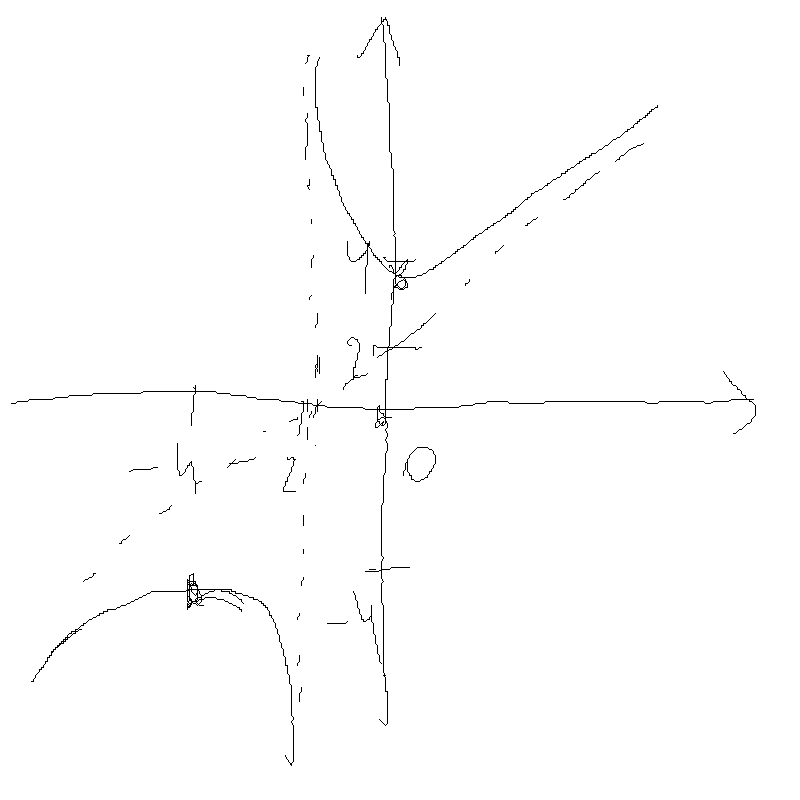
\includegraphics[scale=0.75]{course1/calculus/homeworks/some data/06.8.b.png}
